\documentclass{report}
\usepackage[utf8]{inputenc}
\usepackage[T1]{fontenc}
\usepackage[brazil]{babel}
\usepackage{graphicx}
\usepackage{amsfonts}
\usepackage{amssymb}
\usepackage{amsmath}
\usepackage{multicol}
\usepackage{ifthen}
\newboolean{firstanswerofthechapter}  
\usepackage{xcolor}
\colorlet{lightcyan}{cyan!40!white}
\usepackage{chngcntr}
\usepackage{stackengine}
\usepackage{tasks}
\usepackage{multirow}
\usepackage{float}
\newlength{\longestlabel}
\settowidth{\longestlabel}{\bfseries viii.}
%\settasks{counter-format={tsk[r].}, label-format={\bfseries}, label-width=\longestlabel,
    %item-indent=0pt, label-offset=2pt, column-sep={10pt}}
		
\setcounter{secnumdepth}{0} \setlength{\topmargin}{0cm}
\setlength{\headsep}{-0.3cm} \setlength{\textwidth}{17.5cm}
\setlength{\textheight}{23cm} \setlength{\oddsidemargin}{-0.8cm}
\setlength{\evensidemargin}{0cm} \setlength{\footskip}{-1.5cm}

		
\usepackage[lastexercise,answerdelayed]{exercise}
%\counterwithin{Exercise}{chapter}
%\counterwithin{Answer}{chapter}
%\renewcounter{Exercise}[chapter]
%\newcommand{\QuestionNB}{\bfseries\arabic{Question}.\ }
%\renewcommand{\ExerciseName}{Exercício}
%\renewcommand{\ExerciseHeader}{\noindent\def\stackalignment{l}% code from https://tex.stackexchange.com/a/195118/101651
    %\stackunder[0pt]{\colorbox{cyan}{\textcolor{white}{\textbf{\LARGE\ExerciseHeaderNB\;\large\ExerciseName}}}}{\textcolor{lightcyan}{\rule{\linewidth}{2pt}}}\medskip}
\renewcommand{\ExerciseName}{Exercícios}
\renewcommand{\ExerciseHeader}{\noindent\def\stackalignment{l}% code from https://tex.stackexchange.com/a/195118/101651
    \stackunder[0pt]{\colorbox{cyan}{\textcolor{white}{\textbf{\large\ExerciseName}}}}{\textcolor{lightcyan}{\rule{\linewidth}{2pt}}}\medskip}
%\renewcommand{\AnswerName}{Exercises}
%\renewcommand{\AnswerHeader}{\ifthenelse{\boolean{firstanswerofthechapter}}%
    %{\bigskip\noindent\textcolor{cyan}{\textbf{CHAPTER \thechapter}}\newline\newline%
        %\noindent\bfseries\emph{\textcolor{cyan}{\AnswerName\ \ExerciseHeaderNB, page %
                %\pageref{\AnswerRef}}}\smallskip}
    %{\noindent\bfseries\emph{\textcolor{cyan}{\AnswerName\ \ExerciseHeaderNB, page \pageref{\AnswerRef}}}\smallskip}}
%\setlength{\QuestionIndent}{16pt}

\begin{document}

\vspace*{-2cm}

\begin{center}
\begin{minipage}[s]{2cm}
\hspace{-1.3cm}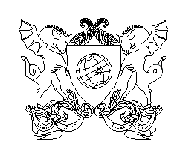
\includegraphics[scale=1.0]{/home/fsbmat/Documentos/GitHub/maf335.github.io/Brasao_UFV/brasaoufv.eps}
\end{minipage}
\begin{minipage}[s]{13cm}
{\begin{center} {\sc \Large Universidade Federal de Vi\c{c}osa}\\
{\sc \large Instituto de Ci\^encias Exatas e Tecnológicas}\\
{\sc \large Campus UFV - Florestal}\\
\end{center}}
\end{minipage}\begin{minipage}[s]{2 cm}
%\includegraphics[width=2 cm]{logoimecc.eps}
\end{minipage}
\end{center}

\vspace{-0.3cm}

%\hline \hline \noindent

%%%%%%%%%%%%%%%%%%%%%%%%%%%%%%%%%%%%%%%%%%%%%%%%%%%%%%%%%%%%%%%%%%%%%%%%%%%

\medskip

\begin{center}

\underline{\underline{{\large{\sc Lista de Álgebra Linear A - Lista 2}}}}

\bigskip

{\large {\bf Prof. Fernando Bastos}}
%\bigskip
%
%%{\sc Data: $19/06/2018$}
\end{center}


\begin{Exercise}
\begin{enumerate}

%%%%%%%%%%%%%%%%%%%%%%%%%%%%%%%%%%%%%%%%%%%%%%%%%%%%%%%%%%%%%%%%
%Exercicio 1
%%%%%%%%%%%%%%%%%%%%%%%%%%%%%%%%%%%%%%%%%%%%%%%%%%%%%%%%%%%%%%%%

\item \label{1lista3} Sejam $u=(-4,3)$, $v=(2,-5)$ e $w=(a,b)$.
\begin{enumerate}
    \item Encontre $a$ e $b$ nos seguintes:
    $(i)$ $w=2u+3v$ \qquad $(ii)$ $w=\frac{2}{5}v$ \qquad $(iii)$
    $u+w=2u-v.$
    \item Represente os vetores acima no plano cartesiano.
    \item Encontre o comprimento dos vetores $u$, $v$ e $w$.
\end{enumerate}

%Exercicio 2
%%%%%%%%%%%%%%%%%%%%%%%%%%%%%%%%%%%%%%%%%%%%%%%%%%%%%%%%%%%%%%%%

\item \label{2lista3} Sejam $u=\left( 4,-1,2\right) $, $v=\left( 3,-2,-4\right) $ e $%
w=(a,b,c)$.
\begin{enumerate}
    \item Encontre $a,b,c$ nos seguintes casos:

    $(i)$ $w-u=v$\qquad $(ii)$ $w=3v$\qquad $(iii)$ $u+w=2u-v.$
    \item  Encontre o comprimento dos vetores $u$, $v$ e $w$.
\end{enumerate}

%%%%%%%%%%%%%%%%%%%%%%%%%%%%%%%%%%%%%%%%%%%%%%%%%%%%%%%%%%%%%%%
Exercicio 3
%%%%%%%%%%%%%%%%%%%%%%%%%%%%%%%%%%%%%%%%%%%%%%%%%%%%%%%%%%%%%%%

%\item \label{3lista3} \item  Encontre um vetor unit\'{a}rio com a
mesma dire\c{c}\~{a}o e o mesmo sentido que $u=(-1,-3).$


%%%%%%%%%%%%%%%%%%%%%%%%%%%%%%%%%%%%%%%%%%%%%%%%%%%%%%%%%%%%%%%
Exercicio 4
%%%%%%%%%%%%%%%%%%%%%%%%%%%%%%%%%%%%%%%%%%%%%%%%%%%%%%%%%%%%%%%

%\item \label{4lista3} \item  Suponha que uma for\c{c}a de $12$
newtons \'{e} aplicada em um objeto ao longo do semi-eixo negativo
dos $x$ e que uma for\c{c}a de $5$ newtons \'{e} aplicada ao longo
do semi-eixo positivo dos $y$. Encontre a intensidade, a
dire\c{c}\~{a}o e o sentido da for\c{c}a resultante. Represente
graficamente.

%%%%%%%%%%%%%%%%%%%%%%%%%%%%%%%%%%%%%%%%%%%%%%%%%%%%%%%%%%%%%%%%%
%Exercicio 5
%%%%%%%%%%%%%%%%%%%%%%%%%%%%%%%%%%%%%%%%%%%%%%%%%%%%%%%%%%%%%%%%

\item \label{5lista3} Suponha que um barco est\'{a} atravessando
um rio na dire\c{c}\~{a}o leste a uma velocidade de $4$
quil\^{o}metros por hora, enquanto a corrente do rio est\'{a}
fluindo na dire\c{c}\~{a}o sul a uma velocidade de $3$
quil\^{o}metros por hora. Encontre a velocidade resultante do
barco. Represente graficamente.

%%%%%%%%%%%%%%%%%%%%%%%%%%%%%%%%%%%%%%%%%%%%%%%%%%%%%%%%%%%%%%%%%
%Exercicio 6
%%%%%%%%%%%%%%%%%%%%%%%%%%%%%%%%%%%%%%%%%%%%%%%%%%%%%%%%%%%%%%%%

\item \label{6lista3}  Em cada item deste exerc\'{i}cio s\~{a}o
dados um espa\c{c}o vetorial
$(V,+,.,%
%TCIMACRO{\TeXButton{real}{\mbox{${\rm I}\!\mbox{\boldmath $ {\rm R}$}$}}}
%BeginExpansion
\mbox{${\rm I}\!\mbox{\boldmath $ {\rm R}$}$}%
%EndExpansion
\Bbb{)}$ e um subconjunto $U$ de $V$. Verifique se $U$ \'{e} um subespa\c{c}%
o do espa\c{c}o vetorial $V$.\newline
$(a)$ $V=%
%TCIMACRO{\TeXButton{real}{\mbox{${\rm I}\!\mbox{\boldmath $ {\rm R}$}$}}}
%BeginExpansion
\mbox{${\rm I}\!\mbox{\boldmath $ {\rm R}$}$}%
%EndExpansion
^{3}$ e $U=\{(x,y,z)\in
%TCIMACRO{\TeXButton{real}{\mbox{${\rm I}\!\mbox{\boldmath $ {\rm R}$}$}}}
%BeginExpansion
\mbox{${\rm I}\!\mbox{\boldmath $ {\rm R}$}$}%
%EndExpansion
^{3};\,x+y+z=0\}.$\newline
$(b)$ $V=%
%TCIMACRO{\TeXButton{real}{\mbox{${\rm I}\!\mbox{\boldmath $ {\rm R}$}$}}}
%BeginExpansion
\mbox{${\rm I}\!\mbox{\boldmath $ {\rm R}$}$}%
%EndExpansion
^{3}$ e $U=\{(x,y,z)\in
%TCIMACRO{\TeXButton{real}{\mbox{${\rm I}\!\mbox{\boldmath $ {\rm R}$}$}}}
%BeginExpansion
\mbox{${\rm I}\!\mbox{\boldmath $ {\rm R}$}$}%
%EndExpansion
^{3};$ $x+y+z\leq 1\}.$\newline
$(c)$ $V=M_{2\times 2}\left(
%TCIMACRO{\TeXButton{real}{\mbox{${\rm I}\!\mbox{\boldmath $ {\rm R}$}$}}}
%BeginExpansion
\mbox{${\rm I}\!\mbox{\boldmath $ {\rm R}$}$}%
%EndExpansion
\right) $ e $U=\left\{ A\in V;\text{ }\det A=0\right\} $.\newline
$(d)$ $V=\Bbb{P}_{3}\left(
%TCIMACRO{\TeXButton{real}{\mbox{${\rm I}\!\mbox{\boldmath $ {\rm R}$}$}}}
%BeginExpansion
\mbox{${\rm I}\!\mbox{\boldmath $ {\rm R}$}$}%
%EndExpansion
\right) \ $e $U=\left\{ p\in
V;\,p=a_{3}x^{3}+a_{2}x^{2}+a_{1}x+a_{0}\text{, }a_{i}\in
\mathbf{Z,}0\leq i\leq 3\right\} $.\newline
$(e)$
$V=\Bbb{P}_{3}\left(
%TCIMACRO{\TeXButton{real}{\mbox{${\rm I}\!\mbox{\boldmath $ {\rm R}$}$}}}
%BeginExpansion
\mbox{${\rm I}\!\mbox{\boldmath $ {\rm R}$}$}%
%EndExpansion
\right) $ e $U=\left\{ p\in V;\,p=ax^{3}+bx+c\right\} .$

%%%%%%%%%%%%%%%%%%%%%%%%%%%%%%%%%%%%%%%%%%%%%%%%%%%%%%%%%%%%%%%%
%Exercicio 7
%%%%%%%%%%%%%%%%%%%%%%%%%%%%%%%%%%%%%%%%%%%%%%%%%%%%%%%%%%%%%%%%

\item \label{7lista3} Determine para que valores de $k$ os vetores do $%
%TCIMACRO{\TeXButton{real}{\mbox{${\rm I}\!\mbox{\boldmath $ {\rm R}$}$}}}
%BeginExpansion
\mbox{${\rm I}\!\mbox{\boldmath $ {\rm R}$}$}%
%EndExpansion
^{3}$ abaixo s\~{a}o L.I. ou L.D.\newline $(a)$ $u=(1,1,2),$
$v=(-1,2,3)$ e $w=(k,-1,1)$\newline $(b)$ $u=(-1,0,7),$
$v=(-4,5,-3k),w=(0,4,-2)$ e $z=(2k,3,1)$.

%%%%%%%%%%%%%%%%%%%%%%%%%%%%%%%%%%%%%%%%%%%%%%%%%%%%%%%%%%%%%%%%
%Exercicio 8
%%%%%%%%%%%%%%%%%%%%%%%%%%%%%%%%%%%%%%%%%%%%%%%%%%%%%%%%%%%%%%%%

\item \label{8lista3} Determine que condi\c{c}\~{o}es $a$, $b$, e
$c$ devem satisfazer para
que o vetor $v=(a,b,c)$ seja combina\c{c}\~{a}o linear dos vetores $%
u=(1,-3,2)$ e $w=(2,-1,1)$.

%%%%%%%%%%%%%%%%%%%%%%%%%%%%%%%%%%%%%%%%%%%%%%%%%%%%%%%%%%%%%%%%
%Exercicio 9
%%%%%%%%%%%%%%%%%%%%%%%%%%%%%%%%%%%%%%%%%%%%%%%%%%%%%%%%%%%%%%%%

\item \label{9lista3} Quais dos seguintes vetores s\~{a}o combina\c{c}\~{a}o
linear de $%
u=\left( 1,2,1,0\right) $, $v=\left( 4,1,-2,3\right) $,\linebreak
$w=\left( 1,2,6,-5\right) $, e $p=\left( -2,3,-1,2\right)
.$\newline $(a)$ $\left( 3,6,3,0\right) \qquad \qquad $\ \ \ $(b)$
$\left( 1,0,0,0\right)
\; $\ \qquad \qquad \ $(c)$ $\left( 3,6,-2,5\right) $\ \qquad \ \qquad \ $(d)$ $%
\left( 0,0,0,1\right) $

%%%%%%%%%%%%%%%%%%%%%%%%%%%%%%%%%%%%%%%%%%%%%%%%%%%%%%%%%%%%%%%%
%Exercicio 10
%%%%%%%%%%%%%%%%%%%%%%%%%%%%%%%%%%%%%%%%%%%%%%%%%%%%%%%%%%%%%%%%

\item \label{10lista3} Determine $\left[ S\right] $, onde
$S=\left\{ \left[
\begin{array}{rr}
1 & 2 \\
-1 & 3
\end{array}
\right] ,\left[
\begin{array}{cc}
2 & 5 \\
1 & -1
\end{array}
\right] ,\left[
\begin{array}{rr}
5 & 12 \\
1 & 1
\end{array}
\right] ,\left[
\begin{array}{rr}
3 & 4 \\
-2 & 5
\end{array}
\right] \right\} .$

%%%%%%%%%%%%%%%%%%%%%%%%%%%%%%%%%%%%%%%%%%%%%%%%%%%%%%%%%%%%%%%%
%Exercicio 11
%%%%%%%%%%%%%%%%%%%%%%%%%%%%%%%%%%%%%%%%%%%%%%%%%%%%%%%%%%%%%%%%

\item \label{11lista3} \item  Os conjuntos abaixo s\~{a}o
linearmente independente ou linearmente dependentes? Justifique
(Fa\c{c}a contas somente quando for realmente
necess\'{a}rio!)\newline $(a)$ ( \qquad )
$\{1,2t,2t+t^{2},2t+2t^{2}\}\subset \Bbb{P}_{2}\left(
%TCIMACRO{\TeXButton{real}{\mbox{${\rm I}\!\mbox{\boldmath $ {\rm R}$}$}}}
%BeginExpansion
\mbox{${\rm I}\!\mbox{\boldmath $ {\rm R}$}$}%
%EndExpansion
\right) $\newline $(b)$ ( \qquad ) $\{\left( 1,1\right) ,\left(
0,1\right) ,\left( -1,5\right) \}\subset
%TCIMACRO{\TeXButton{real}{\mbox{${\rm I}\!\mbox{\boldmath $ {\rm R}$}$}}}
%BeginExpansion
\mbox{${\rm I}\!\mbox{\boldmath $ {\rm R}$}$}%
%EndExpansion
^{2}$\newline $(c)$ ( \qquad ) $\left\{ \left[
\begin{array}{rr}
0 & \quad 0 \\
0 & 0
\end{array}
\right] ,\text{ }\left[
\begin{array}{rr}
\pi & \quad \sqrt{2} \\
\sqrt{3} & 0
\end{array}
\right] ,\text{ }\left[
\begin{array}{rr}
1 & \quad 332 \\
41 & 90
\end{array}
\right] \right\} \subset M_{2\times 2}$\newline
$(d)$ ( \qquad ) $\left\{ (1,3,2,5,7),\left( \frac{1}{2},\frac{3}{2},0,\frac{5%
}{2},\frac{7}{3}\right) \right\} \subset \mathbf{R}^{5}\newline $
$(e)$ ( \qquad ) $\{1\}\subset \mathbf{R}$

%%%%%%%%%%%%%%%%%%%%%%%%%%%%%%%%%%%%%%%%%%%%%%%%%%%%%%%%%%%%%%%%
%Exercicio 12
%%%%%%%%%%%%%%%%%%%%%%%%%%%%%%%%%%%%%%%%%%%%%%%%%%%%%%%%%%%%%%%%

\item \label{12lista3} Coloque $V$ ou $F$, justificando sua
resposta.\newline $(a)$ ( \qquad ) Se $\dim W=3$ e $\mathcal{B}$
\'{e} um subconjunto de $W$ com $4$ vetores ent\~{a}o
$\mathcal{B}$ \'{e} L.D.\newline $(b)$ ( \qquad ) Se $\dim W=3$ e
$\mathcal{B}$ \'{e} um subconjunto de $W$ com $2$ vetores
ent\~{a}o $\mathcal{B}$ \'{e} L.I.\newline $(c)$ ( \qquad ) Todo
subconjunto de um espa\c{c}o vetorial contendo o vetor nulo \'{e}
L.D.\newline $(d)$ ( \qquad ) Se $\dim W=3$ e $v_{1},v_{2}\in W$,
ent\~{a}o $\left[ v_{1},v_{2}\right] \neq W$.\newline $(e)$ (
\qquad ) Se $\dim W=3$ e $v_{1},v_{2},v_{3}\in W$, ent\~{a}o
$\left[ v_{1},v_{2},v_{3}\right] =W$.

%%%%%%%%%%%%%%%%%%%%%%%%%%%%%%%%%%%%%%%%%%%%%%%%%%%%%%%%%%%%%%%%
%Exercicio 13
%%%%%%%%%%%%%%%%%%%%%%%%%%%%%%%%%%%%%%%%%%%%%%%%%%%%%%%%%%%%%%%%

\item \label{13lista3} Verifique que se $u,v\in V$ e $u=\lambda v$
para algum $\lambda \in
\Bbb{\ }%
%TCIMACRO{\TeXButton{real}{\mbox{${\rm I}\!\mbox{\boldmath $ {\rm R}$}$}}}
%BeginExpansion
\mbox{${\rm I}\!\mbox{\boldmath $ {\rm R}$}$}%
%EndExpansion
$, ent\~{a}o $\{u,v\}$ \'{e} L.D.

%%%%%%%%%%%%%%%%%%%%%%%%%%%%%%%%%%%%%%%%%%%%%%%%%%%%%%%%%%%%%%%%
%Exercicio 14
%%%%%%%%%%%%%%%%%%%%%%%%%%%%%%%%%%%%%%%%%%%%%%%%%%%%%%%%%%%%%%%%

\item \label{14lista3} Encontre um sistema homog\^{e}neo cujo
conjunto das solu\c{c}\~{o}es seja gerado por
\[
\{(1,-2,0,3),(1,-1,-1,4),(1,0,-2,5)\}.
\]

%%%%%%%%%%%%%%%%%%%%%%%%%%%%%%%%%%%%%%%%%%%%%%%%%%%%%%%%%%%%%%%%
%Exercicio 15
%%%%%%%%%%%%%%%%%%%%%%%%%%%%%%%%%%%%%%%%%%%%%%%%%%%%%%%%%%%%%%%%

\item \label{15lista3} Suponha que $\{u,v,w\}$ \'{e} um conjunto L.I.. Ent\~{a}o $%
\{u+v,u-v,u-2v+w\}$ \'{e} L.I. ou L.D.?

%%%%%%%%%%%%%%%%%%%%%%%%%%%%%%%%%%%%%%%%%%%%%%%%%%%%%%%%%%%%%%%%
%Exercicio 16
%%%%%%%%%%%%%%%%%%%%%%%%%%%%%%%%%%%%%%%%%%%%%%%%%%%%%%%%%%%%%%%%

\item \label{16lista3} \item  Seja $W=\left\{ \left[
\begin{array}{rr}
2a & \quad a+2b \\
0 & a-b
\end{array}
\right] \text{: }a,b\in
%TCIMACRO{\TeXButton{real}{\mbox{${\rm I}\!\mbox{\boldmath $ {\rm R}$}$}}}
%BeginExpansion
\mbox{${\rm I}\!\mbox{\boldmath $ {\rm R}$}$}%
%EndExpansion
\right\} $.\newline
$(a)$ Mostre que $W$ \'{e} subespa\c{c}o vetorial de $M_{2\times 2}(%
%TCIMACRO{\TeXButton{real}{\mbox{${\rm I}\!\mbox{\boldmath $ {\rm R}$}$}}}
%BeginExpansion
\mbox{${\rm I}\!\mbox{\boldmath $ {\rm R}$}$}%
%EndExpansion
).$\newline $(b)$ $\left[
\begin{array}{rr}
0 & \;-2 \\
0 & 1
\end{array}
\right] \in W$? $\left[
\begin{array}{rr}
0 & \;2 \\
3 & 1
\end{array}
\right] \in W$?\newline $(c)$ Determine uma base para $W$.

%%%%%%%%%%%%%%%%%%%%%%%%%%%%%%%%%%%%%%%%%%%%%%%%%%%%%%%%%%%%%%%%
%Exercicio 17
%%%%%%%%%%%%%%%%%%%%%%%%%%%%%%%%%%%%%%%%%%%%%%%%%%%%%%%%%%%%%%%%

\item \label{17lista3} Seja $\mathbf{W}_{1}=\left\{ A\in M_{3\times 3}(%
%TCIMACRO{\TeXButton{real}{\mbox{${\rm I}\!\mbox{\boldmath $ {\rm R}$}$}}}
%BeginExpansion
\mbox{${\rm I}\!\mbox{\boldmath $ {\rm R}$}$}%
%EndExpansion
);\,A^{\intercal }=A\right\} $, isto \'{e}, $\mathbf{W}_{1}$\'{e}
o conjunto de todas as matrizes sim\'{e}tricas de ordem
$3.$\newline $(a)$ Mostre que $\mathbf{W}_{1}$ \'{e} subespa\c{c}o
vetorial de $M_{3\times
3}(%
%TCIMACRO{\TeXButton{real}{\mbox{${\rm I}\!\mbox{\boldmath $ {\rm R}$}$}}}
%BeginExpansion
\mbox{${\rm I}\!\mbox{\boldmath $ {\rm R}$}$}%
%EndExpansion
).$\newline $(b)$ Determine uma base de $\mathbf{W}_{1}.$

%%%%%%%%%%%%%%%%%%%%%%%%%%%%%%%%%%%%%%%%%%%%%%%%%%%%%%%%%%%%%%%%
%Exercicio 18
%%%%%%%%%%%%%%%%%%%%%%%%%%%%%%%%%%%%%%%%%%%%%%%%%%%%%%%%%%%%%%%%

\item \label{18lista3} Seja $\mathbf{W}_{2}=\left\{ A\in M_{3\times 3}(%
%TCIMACRO{\TeXButton{real}{\mbox{${\rm I}\!\mbox{\boldmath $ {\rm R}$}$}}}
%BeginExpansion
\mbox{${\rm I}\!\mbox{\boldmath $ {\rm R}$}$}%
%EndExpansion
;A^{\intercal }=-A\right\} $, isto\'{e}, $\mathbf{W}_{2}$ \'{e} o
conjunto de todas as matrizes anti-sim\'{e}tricas de ordem
3.\newline $(a)$ Mostre que $\mathbf{W}_{2}$ \'{e} subespa\c{c}o
vetorial de $M_{3\times
3}(%
%TCIMACRO{\TeXButton{real}{\mbox{${\rm I}\!\mbox{\boldmath $ {\rm R}$}$}}}
%BeginExpansion
\mbox{${\rm I}\!\mbox{\boldmath $ {\rm R}$}$}%
%EndExpansion
)$. \newline $(b)$ Determine uma base de $\mathbf{W}_{2}.$

%%%%%%%%%%%%%%%%%%%%%%%%%%%%%%%%%%%%%%%%%%%%%%%%%%%%%%%%%%%%%%%%
%Exercicio 18
%%%%%%%%%%%%%%%%%%%%%%%%%%%%%%%%%%%%%%%%%%%%%%%%%%%%%%%%%%%%%%%%

\item \label{18lista3} Considerando $\mathbf{W}_{1}$ e
$\mathbf{W}_{2}$ os subespa\c{c}os
dos exerc\'{i}cios anteriores mostre que \linebreak $M_{3\times 3}(%
%TCIMACRO{\TeXButton{real}{\mbox{${\rm I}\!\mbox{\boldmath $ {\rm R}$}$}}}
%BeginExpansion
\mbox{${\rm I}\!\mbox{\boldmath $ {\rm R}$}$}%
%EndExpansion
)=\mathbf{W}_{1}+\mathbf{W}_{2}$ e que $\mathbf{W}_{1}\cap \mathbf{W}_{2}$ $%
=\left\{ 0\right\} .$

%%%%%%%%%%%%%%%%%%%%%%%%%%%%%%%%%%%%%%%%%%%%%%%%%%%%%%%%%%%%%%%%
%Exercicio 19
%%%%%%%%%%%%%%%%%%%%%%%%%%%%%%%%%%%%%%%%%%%%%%%%%%%%%%%%%%%%%%%%

\item \label{19lista3} Determine uma base e a dimens\~{a}o do
subespa\c{c}o de $M_{3\times
3}(%
%TCIMACRO{\TeXButton{real}{\mbox{${\rm I}\!\mbox{\boldmath $ {\rm R}$}$}}}
%BeginExpansion
\mbox{${\rm I}\!\mbox{\boldmath $ {\rm R}$}$}%
%EndExpansion
)$ formado por todas as matrizes diagonais.
%
%%%%%%%%%%%%%%%%%%%%%%%%%%%%%%%%%%%%%%%%%%%%%%%%%%%%%%%%%%%%%%%%
%Exercicio 20
%%%%%%%%%%%%%%%%%%%%%%%%%%%%%%%%%%%%%%%%%%%%%%%%%%%%%%%%%%%%%%%%

\item \label{20lista3} Determine uma base e a dimens\~{a}o do
subespa\c{c}o de $M_{3\times
3}(%
%TCIMACRO{\TeXButton{real}{\mbox{${\rm I}\!\mbox{\boldmath $ {\rm R}$}$}}}
%BeginExpansion
\mbox{${\rm I}\!\mbox{\boldmath $ {\rm R}$}$}%
%EndExpansion
)$ formado por todas as matrizes triangulares superiores.

%%%%%%%%%%%%%%%%%%%%%%%%%%%%%%%%%%%%%%%%%%%%%%%%%%%%%%%%%%%%%%%%
%Exercicio 21
%%%%%%%%%%%%%%%%%%%%%%%%%%%%%%%%%%%%%%%%%%%%%%%%%%%%%%%%%%%%%%%%

\item \label{21lista3} Determine a dimens\~{a}o e uma base do
espa\c{c}o solu\c{c}\~{a}o dos seguintes sistemas
homog\^{e}neos:\newline $\left\{
\begin{array}{l}
x+2y+z-3t=0 \\
2x+4y+4z-t=0 \\
3x+6y+7z+t=0
\end{array}
\right. \qquad \qquad \left\{
\begin{array}{l}
x+2y+2z-s+3t=0 \\
x+2y+3z+s+t=0 \\
3x+6y+8z+s+5t=0
\end{array}
\right. \quad $

%%%%%%%%%%%%%%%%%%%%%%%%%%%%%%%%%%%%%%%%%%%%%%%%%%%%%%%%%%%%%%%%
%Exercicio 22
%%%%%%%%%%%%%%%%%%%%%%%%%%%%%%%%%%%%%%%%%%%%%%%%%%%%%%%%%%%%%%%%

\item \label{22lista3} Sejam $U$ e $W$ os subespa\c{c}os do $%
%TCIMACRO{\TeXButton{real}{\mbox{${\rm I}\!\mbox{\boldmath $ {\rm R}$}$}}}
%BeginExpansion
\mbox{${\rm I}\!\mbox{\boldmath $ {\rm R}$}$}%
%EndExpansion
^{4}$ gerados por
\[
\{(1,1,0,-1),(1,2,3,0),(2,3,3,-1)\}\text{ e }%
\{(1,2,2,-2),(2,3,2,-3),(1,3,4,-3)\}
\]
respectivamente. Determine:

$(a)$ $\dim U$;\quad $(b)$ $\dim W$; $(c)$ $\dim (U\cap W)$ e
$(d)$ $\dim (U+W)$

%%%%%%%%%%%%%%%%%%%%%%%%%%%%%%%%%%%%%%%%%%%%%%%%%%%%%%%%%%%%%%%%
%Exercicio 23
%%%%%%%%%%%%%%%%%%%%%%%%%%%%%%%%%%%%%%%%%%%%%%%%%%%%%%%%%%%%%%%%

\item \label{23lista3} Sejam $V=%
%TCIMACRO{\TeXButton{real}{\mbox{${\rm I}\!\mbox{\boldmath $ {\rm R}$}$}}}
%BeginExpansion
\mbox{${\rm I}\!\mbox{\boldmath $ {\rm R}$}$}%
%EndExpansion
^{4}$, $W_{1}=\left\{ \left( a_{1},a_{2},a_{3},a_{4}\right) \in
V;\,a_{1}+a_{3}=0\right\} $ e $W_{2}=\left\{ \left(
b_{1},b_{2},b_{3},b_{4}\right) \in V;\,b_{2}+b_{4}=0\right\} $.
\newline $(a)$ Demonstrar que $W_{1}$ \'{e} subespa\c{c}o de
$V$.\newline $(b)$ Determinar bases de $W_{1}$, $W_{2}$ e
$W_{1}\cap W_{2}$.\newline $(c)$ $W_{1}+$ $W_{2}=V$? Justifique
sua resposta.

%%%%%%%%%%%%%%%%%%%%%%%%%%%%%%%%%%%%%%%%%%%%%%%%%%%%%%%%%%%%%%%%
%Exercicio 24
%%%%%%%%%%%%%%%%%%%%%%%%%%%%%%%%%%%%%%%%%%%%%%%%%%%%%%%%%%%%%%%%

\item \label{24lista3} Considere o subespa\c{c}o $W$ de
$\mathbb{R}^{4}$ gerado pelos
vetores $v_{1}=\left( 1,-1,0,0\right) ,$ $v_{2}=\left( 0,0,1,1\right) ,$ $%
v_{3}=\left( -2,2,1,1\right) ,$ $v_{4}=\left( 1,0,1,0\right) $ . Pede-se:%
\newline
$(a)$ Determine uma base para $W$\textit{. } Qual \'{e} a\textit{\ }$\dim W$%
\textit{?}\newline
$(b)$ O vetor\textit{\ }$u=\left( 2,-3,2,2\right) $\ pertence a\textit{\ }$W$%
\textit{?}\newline
$(c)$ Determine um sistema linear homog\^{e}neo cujo espa\c{c}o das solu\c{c}%
\~{a}o seja\textit{\ }$W$\textit{.}

%%%%%%%%%%%%%%%%%%%%%%%%%%%%%%%%%%%%%%%%%%%%%%%%%%%%%%%%%%%%%%%%
%Exercicio 25
%%%%%%%%%%%%%%%%%%%%%%%%%%%%%%%%%%%%%%%%%%%%%%%%%%%%%%%%%%%%%%%%

\item \label{25lista3} Seja $S=\{u,v,w,r,s,t\}$ um subconjunto
L.I. de um espa\c{c}o vetorial $V$. Seja $R\subset S,$ $R$ com $3$
elementos. Determine $\dim \left[ S\right] $, $\dim \left[
R\right] $, $\dim \left( \left[ S\right] \cap \left[ R\right]
\right) $ e $\dim \left( \left[ S\right] +\left[ R\right] \right)
.$

%%%%%%%%%%%%%%%%%%%%%%%%%%%%%%%%%%%%%%%%%%%%%%%%%%%%%%%%%%%%%%%%
%Exercicio 26
%%%%%%%%%%%%%%%%%%%%%%%%%%%%%%%%%%%%%%%%%%%%%%%%%%%%%%%%%%%%%%%%

\item \label{17lista3} Considere o subconjunto $\gamma =\left\{
\left( 1,0,2\right) ,\left(
0,1,-1\right) ,\left( 1,0,1\right) \right\} $ do $%
%TCIMACRO{\TeXButton{real}{\mbox{${\rm I}\!\mbox{\boldmath $ {\rm R}$}$}}}
%BeginExpansion
\mbox{${\rm I}\!\mbox{\boldmath $ {\rm R}$}$}%
%EndExpansion
^{3}.$ Pede-se:\newline
$(a)$ Mostre que $\mathcal{\gamma }$ \'{e} uma base para o $%
%TCIMACRO{\TeXButton{real}{\mbox{${\rm I}\!\mbox{\boldmath $ {\rm R}$}$}}}
%BeginExpansion
\mbox{${\rm I}\!\mbox{\boldmath $ {\rm R}$}$}%
%EndExpansion
^{3}$ e calcule a matriz mudan\c{c}a da base $\mathcal{\gamma }$ para a base
can\^{o}nica $\mathcal{C}.$\newline
$(b)$ Dado o vetor $u=\left( 1,1,1\right) $ determine suas coordenadas em rela%
\c{c}\~{a}o \`{a} base $\gamma .$

%%%%%%%%%%%%%%%%%%%%%%%%%%%%%%%%%%%%%%%%%%%%%%%%%%%%%%%%%%%%%%%%
%Exercicio 27
%%%%%%%%%%%%%%%%%%%%%%%%%%%%%%%%%%%%%%%%%%%%%%%%%%%%%%%%%%%%%%%%

\item \label{27lista3} No espa\c{c}o vetorial $\Bbb{P}_{2}\left(
%TCIMACRO{\TeXButton{real}{\mbox{${\rm I}\!\mbox{\boldmath $ {\rm R}$}$}}}
%BeginExpansion
\mbox{${\rm I}\!\mbox{\boldmath $ {\rm R}$}$}%
%EndExpansion
\right) $ dos polin\^{o}mios em $t$ de grau menor ou igual a $2$, considere
o seguinte conjunto
\[
\mathcal{B}=\{1,\text{ }1-t,\text{ }(1-t)^{2}\}.
\]
$(a)$ Mostre que $\mathcal{B}$ \'{e} uma base de
$\Bbb{P}_{2}.$\newline $(b)$ Encontre as coordenadas dos seguintes
vetores com rela\c{c}\~{a}o \`{a} base ordenada
$\mathcal{B}$:\newline \qquad \qquad (i) $v=2-3t+t^{2}$; \qquad
\qquad (ii) $w=3-2t.$

%%%%%%%%%%%%%%%%%%%%%%%%%%%%%%%%%%%%%%%%%%%%%%%%%%%%%%%%%%%%%%%%
%Exercicio 28
%%%%%%%%%%%%%%%%%%%%%%%%%%%%%%%%%%%%%%%%%%%%%%%%%%%%%%%%%%%%%%%%

\item \label{28lista3} Seja $V=\left\{ p:\left[ -1,1\right]
\rightarrow
%TCIMACRO{\TeXButton{real}{\mbox{${\rm I}\!\mbox{\boldmath $ {\rm R}$}$}}}
%BeginExpansion
\mbox{${\rm I}\!\mbox{\boldmath $ {\rm R}$}$}%
%EndExpansion
;\,p(x)=a_{3}x^{3}+a_{2}x^{2}+a_{1}x+a_{0}\right\} $ e
\[
S=\left\{ p\in V;\;\,p\left( -1\right) =0\text{ e }p^{\prime }\left(
1\right) =0\right\} .
\]
Mostre que $S$ \'{e} um subespa\c{c}o vetorial de $V.$ Encontre uma base e a
dimens\~{a}o do subespa\c{c}o $S$.

%%%%%%%%%%%%%%%%%%%%%%%%%%%%%%%%%%%%%%%%%%%%%%%%%%%%%%%%%%%%%%%%
%Exercicio 29
%%%%%%%%%%%%%%%%%%%%%%%%%%%%%%%%%%%%%%%%%%%%%%%%%%%%%%%%%%%%%%%%

\item \label{29lista3} Sejam $U$ e $W$ os seguintes subespa\c{c}os do $%
%TCIMACRO{\TeXButton{real}{\mbox{${\rm I}\!\mbox{\boldmath $ {\rm R}$}$}}}
%BeginExpansion
\mbox{${\rm I}\!\mbox{\boldmath $ {\rm R}$}$}%
%EndExpansion
^{4}:$%
\begin{eqnarray*}
U &=&\{(x,y,z,w)\subset
%TCIMACRO{\TeXButton{real}{\mbox{${\rm I}\!\mbox{\boldmath $ {\rm R}$}$}} }
%BeginExpansion
\mbox{${\rm I}\!\mbox{\boldmath $ {\rm R}$}$}%
%EndExpansion
^{4};\text{ }\,y+z+w=0\} \\
W &=&\{(x,y,z,w)\subset
%TCIMACRO{\TeXButton{real}{\mbox{${\rm I}\!\mbox{\boldmath $ {\rm R}$}$}} }
%BeginExpansion
\mbox{${\rm I}\!\mbox{\boldmath $ {\rm R}$}$}%
%EndExpansion
^{4};\text{ }\,x+y=0,\,z=2w\}
\end{eqnarray*}
Determine uma base e a dimens\~{a}o de $U$, $W$, $U\cap W$ e $U+W.$

%%%%%%%%%%%%%%%%%%%%%%%%%%%%%%%%%%%%%%%%%%%%%%%%%%%%%%%%%%%%%%%%
%Exercicio 30
%%%%%%%%%%%%%%%%%%%%%%%%%%%%%%%%%%%%%%%%%%%%%%%%%%%%%%%%%%%%%%%%

\item \label{30lista3} Seja $\mathbf{U}$ o subespa\c{c}o de
$\mathbf{R}^{5}$ gerado por
\[
\left\{ (1,-1,-1,-2,0),(1,-2,-2,0,-3),(1,-1,-2,-2,1)\right\}
\]
e seja $\mathbf{W}$ o subespa\c{c}o gerado por $\left\{
(1,-2,-3,0,-2),(1,-1,-3,2,-4),(1,-1,-2,2,-5)\right\} .$ \newline
$(a)$ Encontre dois sistemas homog\^{e}neos cujos espa\c{c}os das solu\c{c}%
\~{o}es s\~{a}o $\mathbf{U}$ e $\mathbf{W}$, respectivamente.\newline
$(b)$ Encontre uma base e a dimens\~{a}o de $\mathbf{U}\cap \mathbf{W}$.%
\newline
$(c)$ Encontre a dimens\~{a}o de $\mathbf{U}+\mathbf{W}$.

%%%%%%%%%%%%%%%%%%%%%%%%%%%%%%%%%%%%%%%%%%%%%%%%%%%%%%%%%%%%%%%%
%Exercicio 31
%%%%%%%%%%%%%%%%%%%%%%%%%%%%%%%%%%%%%%%%%%%%%%%%%%%%%%%%%%%%%%%%

\item \label{31lista3} Se $\left[ I\right] _{\alpha }^{\beta
}=\left[
\begin{array}{rrr}
1 & 1 & 0 \\
0 & -1 & 1 \\
1 & 0 & \,-1
\end{array}
\right] $ e $\beta $ \'{e} a base can\^{o}nica ordenada de $%
%TCIMACRO{\TeXButton{real}{\mbox{${\rm I}\!\mbox{\boldmath $ {\rm R}$}$}}}
%BeginExpansion
\mbox{${\rm I}\!\mbox{\boldmath $ {\rm R}$}$}%
%EndExpansion
^{3}$, determine a base $\alpha .$

%%%%%%%%%%%%%%%%%%%%%%%%%%%%%%%%%%%%%%%%%%%%%%%%%%%%%%%%%%%%%%%%
%Exercicio 32
%%%%%%%%%%%%%%%%%%%%%%%%%%%%%%%%%%%%%%%%%%%%%%%%%%%%%%%%%%%%%%%%

\item \label{32lista3} Se $\left[ I\right] _{\alpha }^{\beta
}=\left[
\begin{array}{rrr}
1 & 1 & 0 \\
0 & -1 & 1 \\
1 & 0 & \,-1
\end{array}
\right] $ ache \newline $(a)$ $\left[ v\right] _{\alpha }$ onde
$\left[ v\right] _{\beta }=\left[
\begin{array}{r}
-1 \\
2 \\
3
\end{array}
\right] \qquad $ $(b)$ $\left[ v\right] _{\beta }$ onde $\left[
v\right] _{\alpha }=\left[
\begin{array}{r}
-1 \\
2 \\
3
\end{array}
\right] $

%%%%%%%%%%%%%%%%%%%%%%%%%%%%%%%%%%%%%%%%%%%%%%%%%%%%%%%%%%%%%%%%
%Exercicio 33
%%%%%%%%%%%%%%%%%%%%%%%%%%%%%%%%%%%%%%%%%%%%%%%%%%%%%%%%%%%%%%%%

\item \label{33lista3} Sejam $\beta _{1}=\left\{ \left(
2,-1\right) ,\left( 3,4\right) \right\} $, $\beta _{2}=\left\{
\left( 1,0\right) ,\left( 0,1\right)
\right\} $ bases ordenadas de $%
%TCIMACRO{\TeXButton{real}{\mbox{${\rm I}\!\mbox{\boldmath $ {\rm R}$}$}}}
%BeginExpansion
\mbox{${\rm I}\!\mbox{\boldmath $ {\rm R}$}$}%
%EndExpansion
^{2}$. Determine $\left[ I\right] _{\beta _{1}}^{\beta _{2}}$ e $\left[
\left( 5,-8\right) \right] _{\beta _{1}}$.

%%%%%%%%%%%%%%%%%%%%%%%%%%%%%%%%%%%%%%%%%%%%%%%%%%%%%%%%%%%%%%%%
%Exercicio 34
%%%%%%%%%%%%%%%%%%%%%%%%%%%%%%%%%%%%%%%%%%%%%%%%%%%%%%%%%%%%%%%%

\item \label{34lista3} Sejam $\beta =\left\{ \left( 1,0\right) ,\left( 0,1\right) \right\} $%
, $\beta _{1}=\left\{ \left( -1,1\right) ,\left( 1,1\right) \right\} $, $%
\beta _{2}=\left\{ \left( \sqrt{3},1\right) ,\left( \sqrt{3},-1\right)
\right\} $ e $\beta _{3}=\left\{ \left( 2,0\right) ,\left( 0,2\right)
\right\} $ bases ordenadas de $%
%TCIMACRO{\TeXButton{real}{\mbox{${\rm I}\!\mbox{\boldmath $ {\rm R}$}$}}}
%BeginExpansion
\mbox{${\rm I}\!\mbox{\boldmath $ {\rm R}$}$}%
%EndExpansion
^{2}$.\newline $(a)$ Ache as matrizes de mudan\c{c}a de
base:\newline
\qquad \qquad $(i)$ $\left[ I\right] _{\beta }^{\beta _{1}}\qquad $ $(ii)$ $%
\left[ I\right] _{\beta _{1}}^{\beta }$ \qquad $(iii)$ $\left[
I\right]
_{\beta _{2}}^{\beta }\qquad $(iv) $\left[ I\right] _{\beta _{3}}^{\beta }$%
\newline
$(b)$ Quais as coordenadas do vetor $v=(3,-2)$ em rela\c{c}\~{a}o \`{a} base:%
\newline
\qquad \qquad $(i)$ $\beta \qquad $ $(ii)$ $\beta _{1}$ \qquad
$(iii)$ $\beta _{2}\qquad $ $(iv)$ $\beta _{3}$\newline $(c)$ As
coordenadas de um vetor $v$ em rela\c{c}\~{a}o \`{a} base $\beta
_{1}$ s\~{a}o dadas por $\left[ v\right] _{\beta _{1}}=\left[
\begin{array}{l}
4 \\
0
\end{array}
\right] $. Quais s\~{a}o as coordenadas de $v$ em rela\c{c}\~{a}o \`{a} base:%
\newline
\qquad \qquad $(i)$ $\beta \qquad $ $(ii)$ $\beta _{2}$ \qquad
$(iii)$ $\beta _{3}$

%%%%%%%%%%%%%%%%%%%%%%%%%%%%%%%%%%%%%%%%%%%%%%%%%%%%%%%%%%%%%%%%
%Exercicio 35
%%%%%%%%%%%%%%%%%%%%%%%%%%%%%%%%%%%%%%%%%%%%%%%%%%%%%%%%%%%%%%%%

\item \label{35lista3} Sejam $\beta _{1}=\left\{ \left( 1,0\right)
,\left( 0,2\right) \right\} $, $\beta _{2}=\left\{ \left(
-1,0\right) ,\left( 1,1\right) \right\} $ e $\beta _{2}=\left\{
\left( -1,-1\right) ,\left( 0,-1\right)
\right\}$ tr\^{e}s bases ordenadas de $%
%TCIMACRO{\TeXButton{real}{\mbox{${\rm I}\!\mbox{\boldmath $ {\rm R}$}$}}}
%BeginExpansion
\mbox{${\rm I}\!\mbox{\boldmath $ {\rm R}$}$}%
%EndExpansion
^{2}$. \newline $(a)$ Ache\newline
\qquad \qquad $(i)$ $\left[ I\right] _{\beta _{1}}^{\beta _{2}}\qquad $ $(ii)$ $%
\left[ I\right] _{\beta _{2}}^{\beta _{3}}$ \qquad $(iii)$ $\left[
I\right] _{\beta _{1}}^{\beta _{3}}\qquad $ $(iv)$ $\left[
I\right] _{\beta _{1}}^{\beta _{2}}\left[ I\right] _{\beta
_{2}}^{\beta _{3}}$\newline $(b)$ Se for poss\'{i}vel, d\^{e} uma
rela\c{c}\~{a}o entre estas matrizes de mudan\c{c}a de base.

\end{enumerate}

\end{Exercise}

\end{document}